\chapter{Computational methods}
\section{Introduction} % TODO Update from MRes version
Computational techniques are a vital tool in the prediction and characterisation of solid state materials.
Not only can computational methods reduce experimental load by identifying promising material candidates in screening studies, but they can offer atomic scale insights into the structural and transport properties of materials not observable by experiment.

This study primarily uses potentials-based minimisation techniques and Molecular Dynamics (MD), implemented in GULP \cite{Gale2003} and LAMMPS \cite{StevePlimton1995} respectively.
In this chapter, the fundamental concepts and mathematics underpinning these techniques are presented.
Furthermore, an overview of classical interatomic potential fitting strategies are presented to contrast to the work presented herein. %TODO chapter reference
This overview is brief and focuses primarily on techniques used in this report, as more comprehensive reviews are available elsewhere. \cite{Gale2003, Jensen2007, Catlow2013}
Some work presented in this section is derived from the MRes report which led to this project, as the fundamental equations underpinning computational methods remain the same.

\section{Atomistic modelling}
An understanding of the forces atoms experience as a function of their environment is vital to gain insights into the properties of systems of interest.
One class of approaches for calculating the interatomic forces between atoms, \textit{ab initio} techniques, are based on quantum mechanics, and seek to determine electron density as a function of position. Whilst the scale of systems these strategies can be used for is increasing with developments in computational resource available, these techniques remain prohibitively expensive for large systems or systems studied over large time-scales.

In contrast, atomistic techniques seek to express the forces between atoms as a series of empirically derived models, either fitted to experimental or \textit{ab initio} data, which can be cheaply evaluated, allowing for large scale systems to be studied over large time scales. This is particularly important when considering phenomenon which occur over large time scales, such as diffusion. 

\section{Potential models}
All atoms in a system, and their current position, momentum, and oxidation state, give rise to highly complex interactions contributing to the internal energy of the system, which must be enumerated if a perfect atomistic model is to be developed.
%In practice, the complexity of such a model would be too expensive to compute, and infeasible to conceive of a rational physical basis for terms consisting of high numbers of interactions 
%(An equation encompassing all forces arising from 10-body interactions is not easy to determine for example).

Potential models are used to determine the forces in such systems by treating these as a series of discrete isolated interactions which sum to the same overall effect. 
The internal energy of the system can then be given as the sum from one to n-body terms as such:\cite{Gale2003}
\begin{align}
U &=& &\sum_{i = 1} U_i&         &+& &\frac{1}{2}\sum_{i = 1} \sum_{j = 1} U_{ij}&  &+& &\frac{1}{6}\sum_{i = 1} \sum_{j = 1} \sum_{k = 1} U_{ijk}& &+& &\cdots\\
&=& &\sum_{i = 1}^\prime U_i&  &+& &\sum_{i,j = 1}^\prime U_{ij}&                 &+& &\sum_{i,j,k = 1}^\prime U_{ijk}&                           &+& &\cdots
\label{eq:taylor}
\end{align}
With the first term accounting for single-body terms, the second term accounting for those interactions which exist between pairs of bodies and so on.
The primed sum in Equation \ref{eq:taylor} distinguishes between interactions that are enumerated repeatedly, and instead counts each unique interaction only once, hence cancelling the $\frac{1}{N!}$ term.
This expansion is exact if expanded to account for all N-body interactions in a system.

As it is only the low order terms which give rise to the majority of the internal energy of a system, it suffices to truncate this expansion to lower order terms.
Typically, this is limited to two-body terms, although higher order terms are included where these strongly impact the system (e.g. bond angles).
Beyond this, higher order terms are only considered where the calculation of a specific property of interest requires their inclusion.
Three-body interactions are required to calculate phonon distribution curves for example.

Furthermore, as the number of bodies in an interaction increases, it becomes increasingly difficult to find a rational physical basis on which an empirical model can be based. 
 
Single body interactions are implemented to represent an external forcefield being applied to a system, such as the application of an external electric field interacting with charged species.
They are also used in the Einstein model, in which species do not interact with one another, and instead are attached to their lattice sites by a spring term.
Single body terms are not used in the course of this study, but are referenced here for completeness sake.

\newpage
\subsection{Two-body interactions}
The two-body terms in Equation \ref{eq:taylor}: $$\sum_{i,j = 1}^\prime U_{ij}$$ account for the interactions occurring between pairs of atoms or ions in isolation.
As no reference frame is given, these terms are therefore strictly a function of interatomic separation.

It is conventional to further subdivide these two-body interactions into Coulombic (long-range) and short-range terms as so:
\begin{equation}
U_{ij} = \Phi_{Coulombic} + \Phi_{short-range}
\label{eq:two-body}
\end{equation}

The Coulombic term in Equation \ref{eq:two-body} is the potential arising from electrostatic interactions between pairs of charged species:

\begin{equation}
\Phi_{Coulombic} = \frac{q_iq_j}{r_{ij}}
\label{eq:coulombic}
\end{equation}
Where $q_i$ and $q_j$ are the effective charges of the species.
This term is colloquially referred to as the ``long-range'' term, as the non-Coulombic component of these interactions are comparatively tiny beyond a certain range.
It is also typically the dominant component in a system at equilibrium, accounting for around 90\% of the total potential energy in a usual system.\cite{Catlow2013}

The long-range nature of the Coulombic term leads to slow convergence in direct space for a large number of ions.
The \citet{Ewald1921} summation can be used to overcome this shortcoming in periodic systems, by further subdividing the Coulombic interactions into short- and long-range terms.
The short-range components are computed as before, while the long-range terms are solved in reciprocal space.

The nature of a two-body interaction can vary widely dependent on context, with the species, charge, and even local environment impacting the resultant potential.
Depending on the system, covalent interactions, London interactions and electron-pair repulsions may all need to be accounted for with no actual calculation of electron density occurring on which to base the potential.

This can include electron-pair repulsions, London interactions and covalent interactions.
This term can be calculated through the use of tabulated data, or via simple analytical models.
Analytical models are typically empirically derived from experimental data.

The selection of an appropriate model is vital, with considerations including the ionic/covalent nature of the system, availability of experimental data, and computational cost influencing the choice of model.
Furthermore, given potential models are often derived to match experimental data for a given system, ensuring that that same potential is suitable when applied outside of the context in which it was developed is important.

This of course can pose an issue when seeking to study systems where no experimental data is available with which to verify the findings of computational work.
 For ionic systems, the Buckingham Potential form is conventionally used to for two-body interactions:


\begin{equation}
\Phi_{ij} = A\cdot \exp \left(\frac{-r_{ij}}{\rho_{ij}} \right) - \frac{C}{r_{ij}^6}
\label{eq:Buckingham}
\end{equation}

\noindent Other common short range potential models are given in Table \ref{tab:potentialmodels}

\begin{table}[t]
  \centering
  \caption{Common short-range two-body potential models.\cite{Gale2003}}
  \label{tab:potentialmodels}
  \begin{tabular}{@{}lc@{}}
  \toprule
  Potential Model         & Expression     \\
  \midrule
  Buckingham              & $\displaystyle{\Phi_{ij} = A\cdot \exp \left(\frac{-r_{ij}}{\rho_{ij}} \right) - \frac{C}{r_{ij}^6}}$    \\
  \addlinespace
  Harmonic                & $\displaystyle{\Phi_{ij} = \frac{1}{2}k_2(r_{ij}-r_0)^2   + \frac{1}{6}k_3(r_{ij}-r_0)^3    + \frac{1}{24}k_4(r_{ij}-r_0)^4   }$    \\
  \addlinespace
  Lennard-Jones           & $\displaystyle{\Phi_{ij} = \left(\frac{A}{r_{ij}^m} \right) - \left( \frac{B}{r_{ij}^n}\right)}$   \\
  \addlinespace
  Morse                   & $\displaystyle{\Phi_{ij} = D_e \left((1- \exp(-a(r_{ij} - r_0)))^2           -1\right) }$    \\
  \bottomrule
  \end{tabular}
\end{table}

\vspace{-5pt}
\paragraph{Finite-range implementation}
As the name suggests, the short-range terms dominate in the short-range, but the force arising from these interactions decreases rapidly with increasing interatomic distance.
To decrease the computational expense, a threshold radius is defined beyond which all forces are assumed to be zero.
The selection of this threshold is important, as the computational expense is of $O(r_t^2)$, so the shorter this radius the less expensive the simulation, whereas too small a radius will result in a change in the simulation result and decrease in model quality.

In order to prevent this strategy introducing discontinuity into the system, additional terms are added to smoothly reduce the interatomic potential and associated energy derivatives to zero at the threshold radius. %TODO rephrase


\subsection{Three-body interactions}
The nature of three-body terms are dependant on the interactions between three ions or atoms.
These can be interpreted as bond pair repulsions or as a charge dispersion between three bodies in covalent and ionic interpretations respectively.
This term is small relative to the two-body terms, and is usually only included when high degrees of accuracy are required, or for the calculation of properties dependent on three-body interactions such as phonon distribution curves.

A commonly used three-body potential is the harmonic model:
\begin{equation}
  U_{ijk} = \frac{1}{2}k_2(\theta-\theta_0)^2   + \frac{1}{6}k_3(\theta-\theta_0)^3    + \frac{1}{24}k_4(\theta-\theta_0)^4
  \label{eq:threebody}
\end{equation}

In this model, an equilibrium angle is assigned to a bond pair, and any deviations from this angle increase the potential energy of the system.

%\subsection{Lattice energy}
%The lattice energy is simply the energy of formation of a given lattice.
%As temperature is not explicitly considered in GULP, the lattice energy is simply the internal energy.
%Substituting Equations \ref{eq:two-body} to \ref{eq:threebody} into Equation \ref{eq:taylor} yields the following:
%\begin{equation}
%U = \overbrace{\sum_{ij} \frac{q_iq_j}{r_{ij}}}^\text{Coulombic} + \overbrace{\sum_{ij} \Phi_{ij}(r_{ij})}^\text{Short range} + \overbrace{\sum_{ijk} U_{ijk}(r_{ijk})}^\text{Three-body terms}
%\end{equation}


\subsection{Polarizability}
The electron distribution surrounding an atom or ion will shift according to the local environment in which it exists, effectively allowing the internuclear and electronic interactions to partially decouple.
A rigid ion model, in which species are modelled as point charges, does not capture this behaviour, defreasing the accuracy of models using it.
This is a particularly important behaviour when studying ion migration, and so a failure to account for this behaviour can negatively impact the accuracy of results obtained.

An early model of ion polarisation is the point polarisable ion model (PPI), in which the dipole moment of an ion ($\mu$) is directly proportional to the strength of the electric field in which it sits(E):
\begin{equation}
\mu = \alpha E
\end{equation}
Whilst computationally inexpensive and easily extensible to higher order polarizabilities (i.e. quadrupolar systems), this model performs poorly when handling dynamic lattice properties.
It also poorly predicts dielectric constants, which is easily measurable experimentally and thus a useful criteria for model validation.

This shortcoming can be rationalised by the failure to account for the polarisation of adjacent ions, that is, that neighbouring species being polarised impacts the local electric field and serves to dampen polarisation overall.
Consequently, this model tends to overestimate dielectric constants if tuned to accurately predict another physical property (e.g. elastic constants).


\begin{figure}[ht]
  \centering
  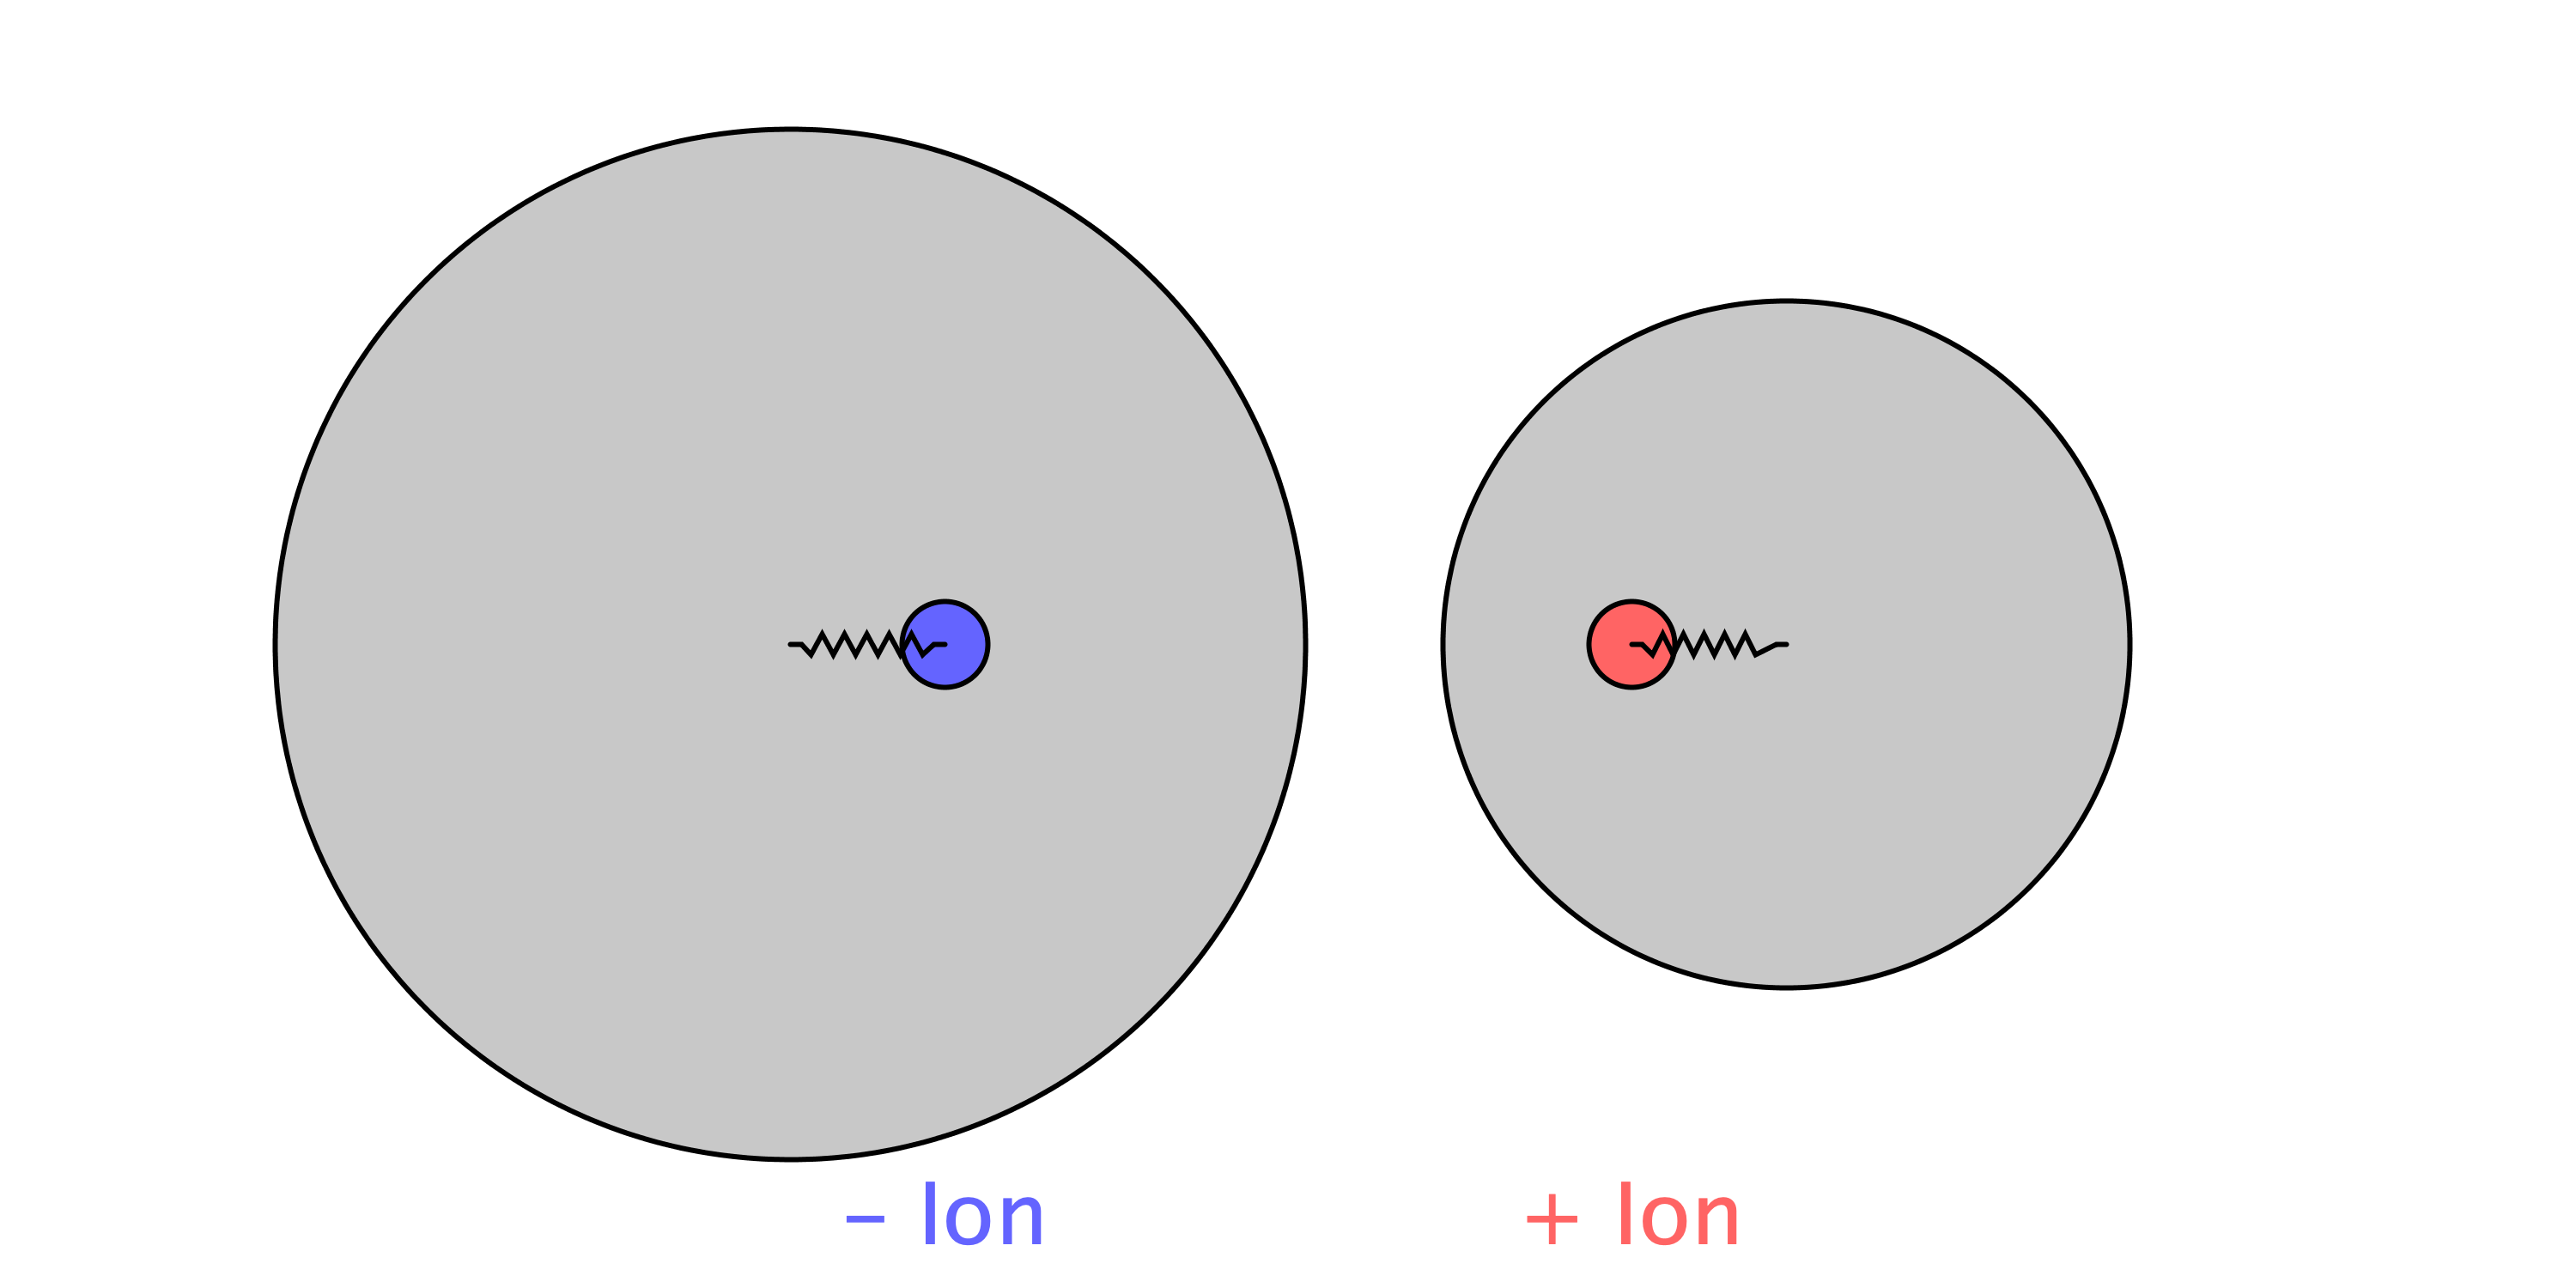
\includegraphics[width=\linewidth]{figures/coreshell/coreshell}
  \caption[Simple schematic of the shell model of polarisability.]{Simple schematic of the shell model of polarisability. The valence electron shells (grey) are attached to the ion core by a harmonic spring, and are displaced by nearby charged species or net electric fields.}
\end{figure}
The shell model\cite{Dick1958} is another computationally inexpensive model of polarisation which accounts for polarisation coupling, thus overcoming a key limitation of the PPI model.
Polarisation coupling is modelled by treating the valence electron cloud as a shell connected to the ionic core by a harmonic spring.
The core represents the nucleus and core electrons of the ion, accounting for the majority of the mass of the ion, while the shell is represents the polarisable valence electrons.
The mass of the shell is treated as zero in non-dynamical systems (i.e. in structural optimisation, Section \ref{sec:minimization}) where the solver strategies are able to handle zero-mass species without instability.
In the case of dynamic systems (i.e. Molecular dynamics, Section \ref{sec:MD}), the shell is assigned a small portion of the overall mass to provide a degree of inertia and remove the need for prohibitively small time-steps.

By allowing the displacement of valence electrons from the ion core, an effective dampening of the polarisation occurs, offering better agreement with experiment.

The charges assigned to the core and shell respectively must sum to that of the point charge it replaces, but the values of these and the spring constant are typically empirically derived.
This polarisation model generally gives good agreement with experiment for ionic halides and oxides.


\section{Partial occupancies}
Partial occupancies can occur in mixed ion systems, where several ions can occupy the same site.
The simplest technique for addressing this situation is the use of a supercell, in which each site is assigned a given ion so as to achieve the desired stoichiometry.
This is possible for simple systems, but in complex crystal structures this is not a viable strategy.

This is in part due to the huge number of potential configurations possible in such systems.
For example, randomly distributing 50 ions at 100 non equivalent lattice sites yields $\frac{100!}{50!\cdot50!} = 10^{29}$ distinct systems.

An alternate strategy in dealing with partial occupancies is to utilise the mean field approximation.
In this approach, each atom or ion is assigned an occupancy at a given site.
The interatomic potentials are calculated as usual, and scaled relative to the occupancy of that site:
$$
U_{ij} = o_io_jU_{ij}
$$
This allows for the average potential to be calculated.
This technique is useful for calculating structural properties, but care should be taken when determining thermodynamic data where the averaging of distinct energy barriers may lead to inaccuracy.

\section{Polarizability}

An early model of ion polarisation is the point polarisable ion model (PPI), in which the dipole moment of an ion ($\mu$) is directly proportional to the strength of the electric field (E):
\begin{equation}
\mu = \alpha E
\end{equation}

This model is useful due to ease of extension to high order polarisabilites (quadrupoles for example).
Whilst of interest due to being computationally inexpensive, this model is inaccurate when calculating dynamical properties of lattices (e.g. phonon dispersion curves) and fails to accurately predict dielectric constants.

This is attributable to a lack of consideration for coupling between polarisation and short term repulsions. That is to say that the polarisation of electron clouds of neighbouring ions increases the overlap between electron clouds and acts to dampen the overall effect.

As such, simulations using this approach to accurately predict elastic constants will overestimate the dielectric constant.

\begin{figure}[ht]
  \centering
  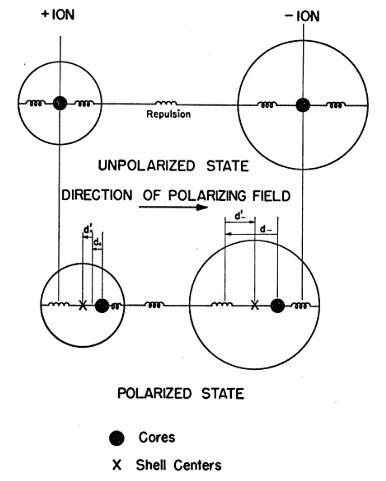
\includegraphics[width=0.4\linewidth]{figures/shell}
  \caption[Schematic of the shell model of polarisability.\cite{Dick1958}]{Schematic of the shell model of polarisability.\cite{Dick1958} The valence electron shell is held to the ion core by a harmonic spring, and can be displaced by other charged species or electric fields.}
\end{figure}
The shell model\cite{Dick1958} is another simple model of polarisation which accounts for polarisation coupling, thus overcoming a key limitation of the PPI model.
Polarisation coupling is modelled by treating the valence electron cloud as a shell of zero mass connected to the ionic core by a harmonic spring.

By allowing the displacement of valence electrons from the ion core, an effective dampening of the polarisation occurs, offering better agreement with experiment.
Potential models are developed individually for shell and core interactions between nearby ions, allowing displacement of the shell from the core.


While simple, this model performs well for the prediction of ionic halides and oxides.
\section{Energy minimisation}
\subsection{The configuration space}
For every ion in a system, the internal energy varies as a function of its position in space.
Given that the introduction of additional ions will impact the energy associated with other ions as well as its own, it is not sufficient to define an internal energy as a 3-space.
Instead, the internal energy of an system containing $n$ ions is a $3n$ dimensional function.
We define the vector of positions of ions within this configurational space as $x$.

Whilst possible for a system to occupy any position within a configurational space, it will always tend towards more thermodynamically favourable states.
As such, it is necessary to establish a method to identify $x$ such that $U(x)$ is minimised if the system being studied is to be of any real-world significance.

Whilst the previous sections in this chapter have defined means of calculating the internal energy of an arbitrary configuration, they offer no insight into the likelihood of that system existing.
It is only by comparing $U(x)$ with adjacent systems in the $3n$ dimensional configurational space that local stability can be established.


As an aside, it is worth noting that assessment of locally adjacent configurations can only identify local minima.
Finding global minima is a problem for which no sure-fire solution exists, beyond computationally expensive brute-force searches.
A number of well-established techniques which improve upon brute-force methods do exist, including Monte-Carlo methods,\cite{Allan2001} Molecular Dynamics (MD), or genetic algorithms. \cite{Barnes1992}

These techniques are not utilised in this study, as local minimisation techniques yield equivalent results so long as initialised near the global minima in the configuration space.
Experimental data can be used to provide initial conditions known to correspond to viable systems, and is widely available for lithium metal phosphates due to academic interest surrounding these materials in recent years.

\subsection{Gradient-based methods}

For a position $x$ in the configurational space, the internal energy of a system can be expanded into a Taylor series:
\begin{equation}
  U(x+\delta x) = U(x) + \frac{\partial U}{\partial x} \delta x + \frac{1}{2!} \frac{\partial ^2 U}{\partial x^2}(\delta x)^2 \cdots
\end{equation}

Truncating this equation at the first derivative yields the energy of a configuration $U(x)$, and a derivative vector $g$, indicating directions in the configuration space in which the energy reduces.

\subsubsection{Steepest descent}
In this method, the position $x$ is updated by:
\begin{equation}
x_{p+1} = x_p + g^p\delta
\end{equation}

with $\delta$ typically being determined using line searches.
The gradient matrix is then recalculated for the new position, and the procecure is repeated until convergence is achieved.

Whilst each step in this method is inexpensive computationally, there is no theoretical limit to how many steps will be required to achieve convergence.
This method also requires recalculation of the gradient vector at each step, and cannot make use of information from previous iterations.

\subsubsection{Conjugate gradients}
The conjugate gradients method optimizes in a single dimension on each step, with subsequent steps taken orthogonal to past search vectors.
This converges in $N$ steps for an $N$ dimensional quadratic search space.

Expansion of the Taylor series to include a second derivative term (and thus, a Hessian matrix $H$), allows a system to be solved by the Newton-Raphson method by:
$$
\Delta x = -H^{-1}g
$$

This is exact if close to the minima, although approximate with increasing distance from the minima.
Employing the steepest descent approach initially, followed by the conjugate gradient methods offers both rapid and bounded convergence to a local minima.


As numerical techniques are being utilised, with ionic coordinates and energies being updated iteratively, it is possible to solve to a degree of precision far beyond that which is either experimentally measurable or remotely useful.
As such, simulations are typically deemed to have converged when the change in energy and ionic coordinates between iterations is below a given threshold value.
The default convergence criteria in GULP are used in this study, with any results presented having converged to at least that degree of precision.

\section{Point defects}
The techniques above are well suited for handling perfect systems, but fail to account for the numerous deviations from perfect crystal structures which occur in real systems.
These defects usually exist in small quantities, but their presence can drastically impact the properties of the material.
As an example, the doping of silicon with boron or phosphorous gives rise to p- and n-type semiconductors respectively.
The presence of excess electrons or electron holes is the basis of the main operating principle of transistors.
Defects strongly influence Li-ion migration rates through electrode materials and are therefore of interest for characterising battery materials.

Whilst the atomistic modelling techniques already discussed are appliciable in the generic case (as can be demonstrated by their suitability when applied to a P1 symmetry group), they have thus far only been discussed in the context of bulk systems.

An overview of defect types, as well as the formalisms used in defining defect formation, is given in the appendix.

\subsection{Mott-Littleton method}
The Mott-Littleton method allows for the modelling of a defect, or multiple defects, at infinite dilution.
This technique is used extensively in literature\cite{Fisher2008} and offers good agreement with experimental data.

Using a relaxed perfect crystal structure as an initial condition, defect(s) are introduced as a perturbation to this system and the system is once more allowed to relax.
The difference in energy of the two systems can be directly attributed to the presence of the defect, and is thus the energy required to allow formation of that defect.
As the introduction of a single point defect removes symmetry from the system, a periodic approach is not appropriate, nor is the consideration of an infinite system.

Instead, concentric spherical regions centred about the defect are defined, and only species which fall within these regions are modelled.
A schematic illustrating these regions is shown in Figure \ref{fig:mott}. 

\begin{figure}
  \centering
  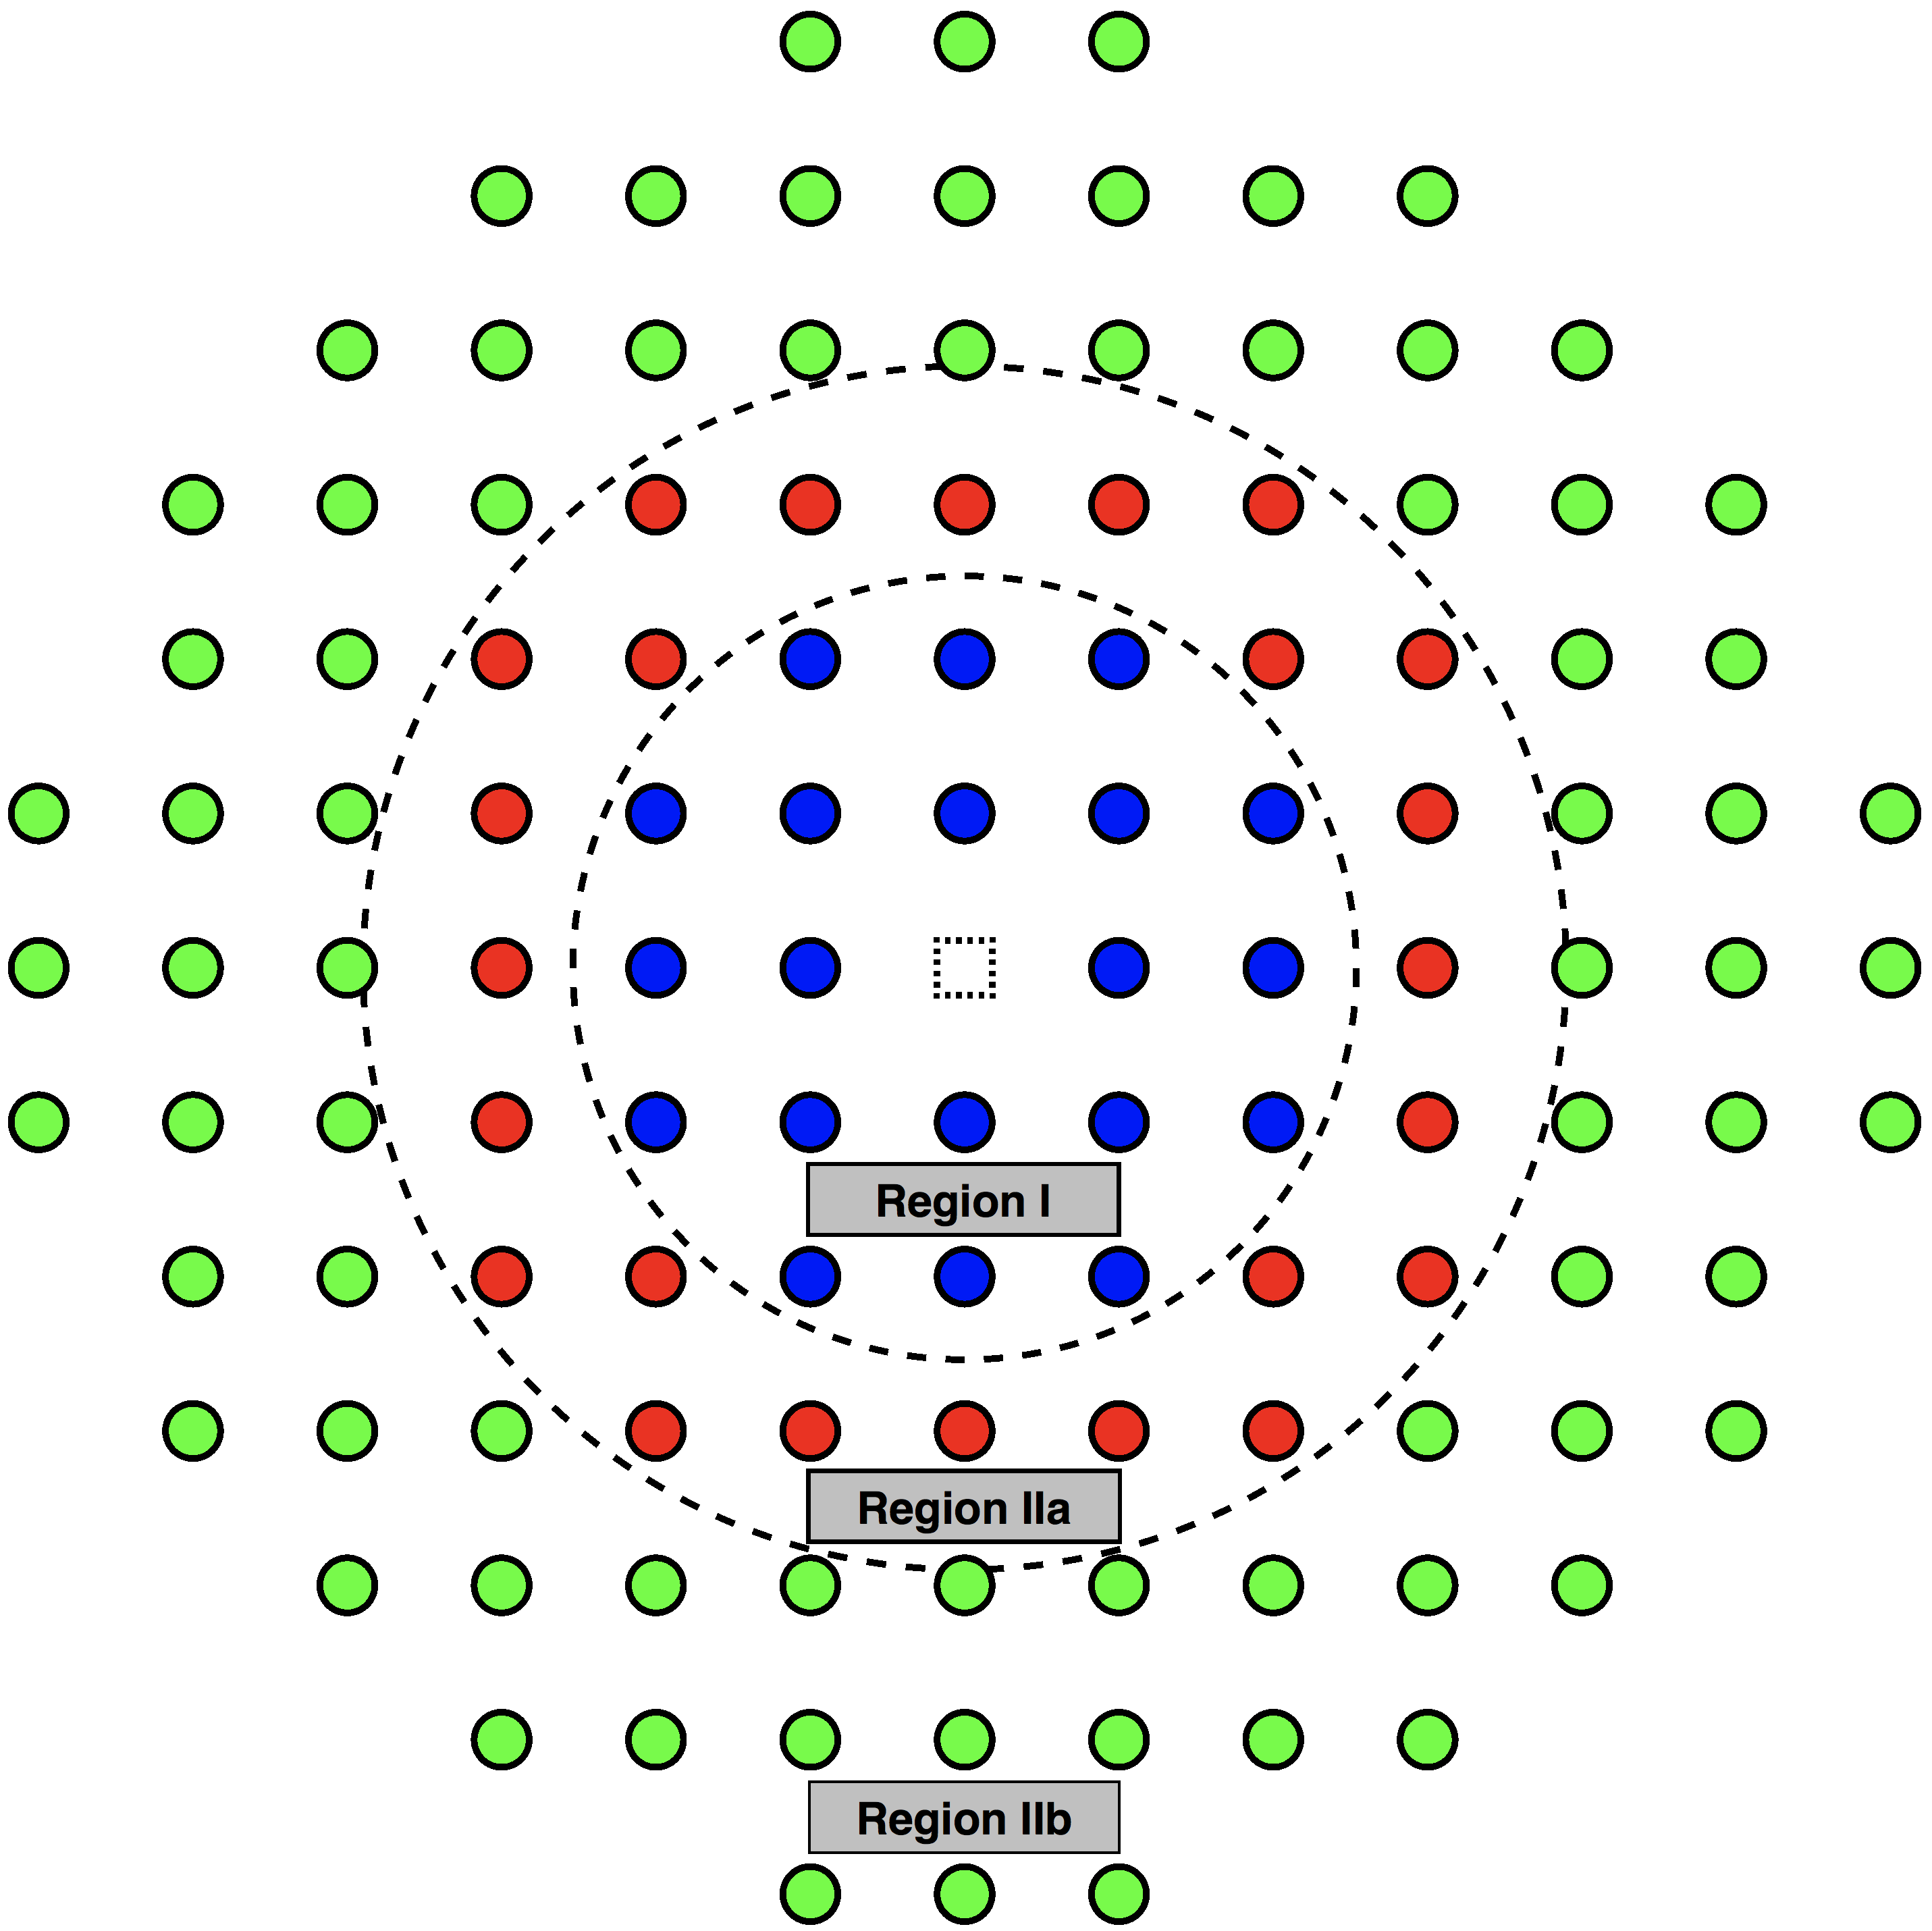
\includegraphics[width = 0.9\linewidth]{figures/Mott-Littleton}
  \caption[Schematic illustrating the regions employed in the Mott-Littleton method.]{Schematic illustrating the regions employed in the Mott-Littleton method. Ions in region I are modelled explicitly due to their proximity to the defect. Region IIb ions are modelled using a continuum method whereas those in region IIa use a harmonic relationship which smooths the transition from explicit to implicit modelling.}
  \label{fig:mott}
\end{figure}

Region I contains those ions closest to the defect.
Their proximity to the defect means it is not feasible to accurately model the impact of the defect on these species with any simple approximations, so they are instead modelled explicitly using interatomic potentials and relaxed using appropriate numerical methods.
Whilst numerical techniques such as the conjugate gradient method can be used to efficiently relax the ions in this region, the 1000 ions which typically constitute region I each with 3 spatial dimensions to be relaxed in yield a 3000 dimensional system of equations to be minimised.
The computational cost is of $O(n!)$ for an n ion system, and so minimising radius to reduce n is highly desirable.

Region II is composed of ions whose energy is not calculated explicitly, but instead through analytical techniques.
It is further subdivided into regions IIa and IIb.
Region IIb, the outermost region, is too distant to be impacted by short range interactions with the defect.
As such, the defect interactions are purely coulombic, and can be modelled implicitly using a dielectric continuum.
The magnitude of the force experienced is a function of the net charge of the defect as well as the distance from the defect center.


Ions in region IIa are modelled as having harmonic interactions, with an energy cost associated with displacing region IIa species from their location in the perfect system.
This region serves to smooth the transition between the explicitly modelled region I and the implicitly modelled region IIb, preventing discontinuities in the energy profile.

The success of this technique relies upon selection of radii such that discontinuities do not occur between regions.
Selection of radii intervals greater than the cut-off values imposed on short range interatomic potentials can achieve this.
In other words, region IIa should be large enough such that no species in region I have any short range interactions with species in region IIb.

It is also important that convergence is achieved, so the radius of region I and region IIa should be increased independently until the defect energy observed converges.
Given the rapid increase in computational cost associated with increasing region sizes (especially region I), the radii selected should be as small as possible whilst not sacrificing accuracy.

\subsection{Supercell approach}
Supercell methods simply take a large supercell of the repeating crystal unit and add a defect to this supercell.
The cell is then modelled as before, with the supercell repeating ``infinitely''.
This approach is limited in that in order to model low defect concentrations, a huge supercell is required.

The supercell approach is therefore more suited to the calculation of systems with high defect concentrations.
As the supercell method differs little from the bulk method beyond initialisation methods, it will not be discussed at length.

The primary limitation of this method is that the supercell must be large enough for convergence to occur, particularly when modelling highly charged species whose coulombic interactions are significant at a large range.

\subsubsection{Symmetry optimisation}
By their nature, crystal structures contain a number of symmetry elements.
In many cases, a number of interactions will be equivalent, enabling the number of computationally expensive operations to be reduced by simply treating some interactions as being equivalent and calculating them once rather than several times.

The addition of defects to a system reduces the overall symmetry of the structure, but there often still exist some symmetry elements.
Symmetry optimised algorithms are automatically implemented where appropriate in GULP.

\newpage

